\documentclass[aspectratio=169]{beamer}

\usepackage[utf8]{inputenc}
\mode<presentation>
{
  \usetheme{Darmstadt}      % or try Darmstadt, Madrid, Warsaw, ...
  \usecolortheme{beaver} % or try albatross, beaver, crane, ...
  \usefonttheme{serif}  % or try serif, structurebold, ...
  \setbeamertemplate{navigation symbols}{}
  \setbeamertemplate{caption}[numbered]
  \setbeamertemplate{footline}[frame number]
  \setbeamertemplate{headline}{}
} 
\usepackage{graphicx}
\usepackage[english]{babel}
\usepackage[utf8]{inputenc}
\usepackage[T1]{fontenc}
\usepackage{bm}
\usepackage{amssymb}
\usepackage{amsmath}
\usepackage{bm}
\usepackage{leftidx}
\usepackage{mathtools}
\usepackage{tikz}
\usepackage{gensymb}
\usepackage{listings}
\pdfsuppresswarningpagegroup=1

\begin{document}
\AtBeginSection[]{
  \begin{frame}
  \vfill
  \centering
  \begin{beamercolorbox}[sep=8pt,center,shadow=true,rounded=true]{title}
    \usebeamerfont{title}\insertsectionhead\par%
  \end{beamercolorbox}
  \vfill
  \end{frame}
}

\title[Your Short Title]{Control of a Hurricane Hunting Aircraft}
\author{Corey Spohn, Jacob Pelster, Rachel Oliver, and Zvonimir Stojanovski}
\institute{MAE 6780 Multivariable Control Theory}
\date{\today}

\begin{frame}
  \titlepage
\end{frame}

\begin{frame}{Model Predictive Control (MPC)}
    \begin{itemize}
        \item Quadratic cost function with a finite horizon
        \begin{eqnarray*}
        J = & \int_0^{T_{p}} \! [\mathbf{x}(t_{i}+\tau|t_{i})^T\mathbf{Q}\mathbf{x}(t_{i}+\tau|t_{i}) +\Dot{\mathbf{u}}(\tau)^T\mathbf{R}\Dot{\mathbf{u}}(\tau)] \, \mathrm{d}\tau 
        \end{eqnarray*}
        \item Incremental control implementation\\
            $ \mathbf{u}(t\rightarrow{t+1}) = -\mathbf{K}_{mpc}*\mathbf{x}(t)$
    \end{itemize}
    \begin{figure}
        \centering
        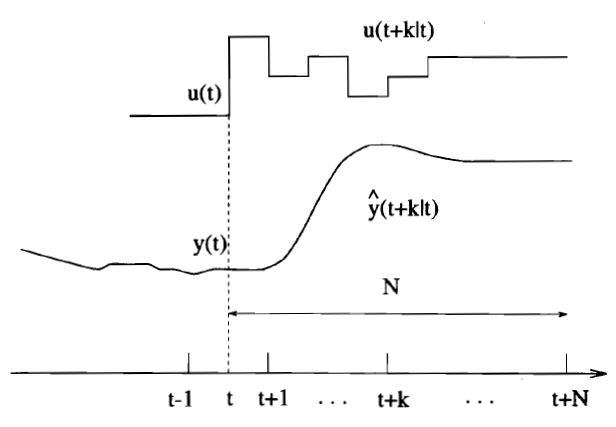
\includegraphics[width=0.6\textwidth]{MPC_Premise.PNG}
    \end{figure}
\end{frame}

\begin{frame}[t]
    \frametitle{MPC Theory}
    %\framesubtitle{subtitle}
    Model predictive control is a fairly broad field of controls, all of which have the following
    \begin{enumerate}
        \item Using a model to predict future outputs
        \item Calculating control inputs using the predicted future outputs and a cost function
        \item Applying the first step of the control input calculated, observing the true output at
            the step, moving the time horizon forward one step, and repeating
    \end{enumerate}
    
\end{frame}

\begin{frame}[t]
    \frametitle{MPC in MATLAB}
    %\framesubtitle{subtitle}
    \begin{itemize}
        \item Requires a discrete-time, delay-free, state-space system plant
        \item 
    \end{itemize}
\end{frame}

\begin{frame}[t]
    \frametitle{Sliding Mode Control}
    %\framesubtitle{test}
    %Sliding Mode Control
    \begin{itemize}
        \item Want to confine state $\mathbf{x}$ to surface $\boldsymbol{\sigma}(\mathbf{x})=\mathbf{0}$ (``sliding surface'') on which system is stable
        \item Control proportional to $\mathrm{sgn}(\boldsymbol{\sigma})$ brings state to sliding surface in finite time (but often better to use sigmoid function to avoid ``chatter'')
        \item Stability conditions depend only on bounds of system dynamics
        \item Can be combined with Model Predictive Control
    \end{itemize}
\end{frame}
\end{document}
